\section{Durchführung}
\label{sec:Durchführung}
\begin{figure}
  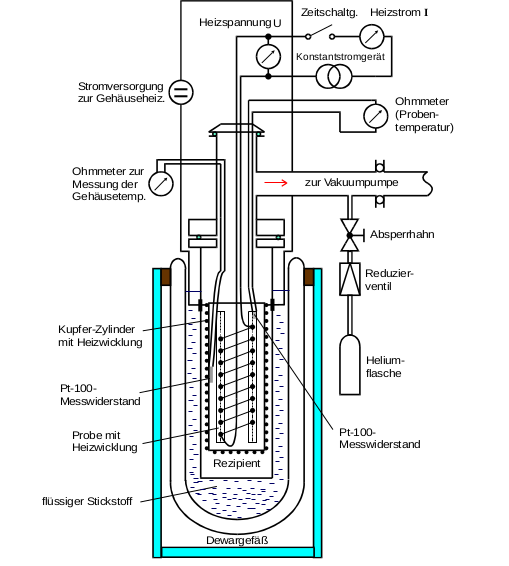
\includegraphics[width=\textwidth]{Aufbau.png}
  \caption{Versuchsaufbau\cite{V47}}
    \label{fig:Aufbau}
\end{figure}
Das Experiment wird in Abbildung \ref{fig:Aufbau} dargestellt.
Die Kupferprobe befindet sich in einem Kupferzylinder, welche beide
jeweils von einer Heizwicklung umschlossen werden.
Der Kupferzylinder wird von einem Rezipienten umschlossen
und der Rezipient wird wiederum in ein Dewargefäß gelegt.
Zur Minimierung der Strahlungsverluste wird in dem
Rezipienten zunächst ein Vakuum mithilfe einer Pumpe erzeugt.
Anschließend wird Helium aus einer Heliumflasche eingelassen.
Mithilfe eines Druckmessgerätes wird gewährleistet, dass das Helium wieder Athmosphärendruck erreicht.
Zur Kühlung der Probe, des Zylinders und des Rezipienten wird als nächstes flüssiger Stickstoff
aus einer speziellen Stickstoffflasche in das Dewargefäß gegossen.
Die Temperaturen des Kupferzylinders und der Probe werden jeweils mithilfe eines Ohmmeters gemessen,
welcher den temperaturabhängegen Widerstand anzeigt.
Nach einer Wartezeit von etwa einer Stunde sind der Zylinder und die Probe auf eine Temperatur von
$80 \, \si{\kelvin}$ abgekühlt und weisen daher beide in etwa den selben Widerstand am Ohmmeter auf.
Gelegentlich muss flüssiger Stickstoff ins Dewargefäß nachgefüllt werden, wenn bereits
so viel Stickstoff verdampft ist, dass der Rezipient teilweise frei liegt,
um eine vollständige und gleichmäßige Kühlung des Rezipienten zu gewährleisten.
Über die Heizwicklung wird sowohl der Probe als auch dem Kupferzylinder eine definierte elektrische Energie hinzugefügt.
Die Stromstärke wird an einem Konstantstromgerät eingestellt und die Spannung an einem Voltmeter abgelesen.
Der Kupferzylinder wird ebenfalls mit elektrischem Strom geheizt, wobei darauf geachtet werden  muss,
dass die Temperaturen der Probe und des Zylinders gleich bleiben, um Wärmestrahlungsverluste zu vermeiden.
Über die Ohmmeter wird die Temperatur kontrolliert.
Falls bei der Messung die Temperaturen abweichen, wird die Stromstärke, welche an der Probe anliegt,
entsprechend variiert, sodass die Temperaturen sich wieder annähern.
Bei der Messung wird nach jedem Zeitintervall von $5 \, \si{\min}$ der elektrische Widerstand
sowie die während des Zeitintervalls anliegende Stromstärke und Spannung an der Probe und des Zylinders aufgeschrieben,
woraus in der Auswertung die hinzugefügte Energie und die Temperaturerhöhung ermittelt werden kann.
Dabei sollte während eines Messintervalls die Stromstärke nicht verändert werden,
um die zugefügte Energie genau berechnen zu können.
